\chapter{Model Evaluation Results}

\section{RIRD ranking results}
\begin{table}[H]
\centering\small
\caption{RIRD ranking results for the principal configurations.}
\label{tab:final-results}
\begin{tabular}{@{}lcccc@{}}
\toprule
Model & Unit and aggregation & nDCG@10 & MAP & MRR\\
\midrule
BM25 & review, top-10 mean & 0.634 & 0.576 & 0.762\\
Dense & review, top-10 mean & 0.668 & 0.608 & 0.760\\
BM25 & sentence, top-10 mean & 0.609 & --- & ---\\
\textbf{Dense} & \textbf{sentence, top-10 mean} & \textbf{0.682} & \textbf{0.618} & \textbf{0.773}\\
RIRD fine-tuned reference & --- & --- & 0.626 & ---\\
\bottomrule
\end{tabular}
\end{table}

The proposed dense sentence model is the strongest tested configuration, reaching nDCG@10
0.682, MAP 0.618 and MRR 0.773. It approaches the supervised RIRD reference MAP of 0.626
without domain-specific fine-tuning. The review-level dense model reaches 0.668/0.608,
showing that sentence granularity improves the selected top-$k$ configuration. Conversely,
sentence-level BM25 is weaker than review-level BM25, demonstrating that finer granularity
does not benefit every representation.

\begin{figure}[H]
\centering
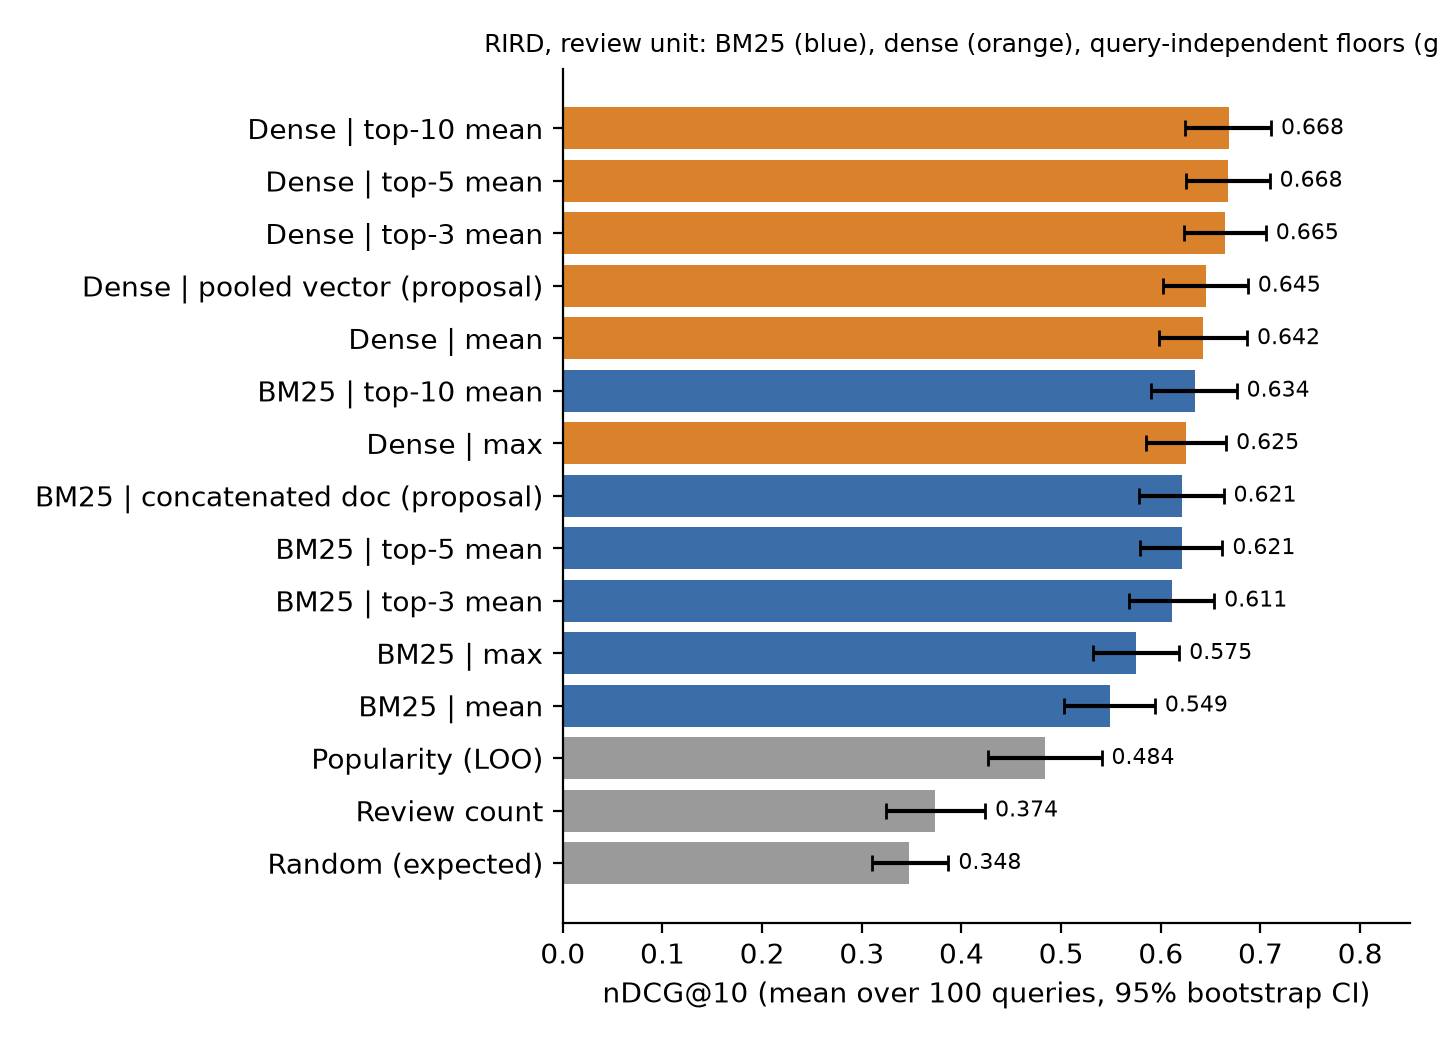
\includegraphics[width=0.88\linewidth]{figures/v2_ndcg_ci.png}
\caption{Review-level nDCG@10 with 95\% bootstrap confidence intervals.}
\label{fig:ndcg}
\end{figure}

\begin{figure}[H]
\centering
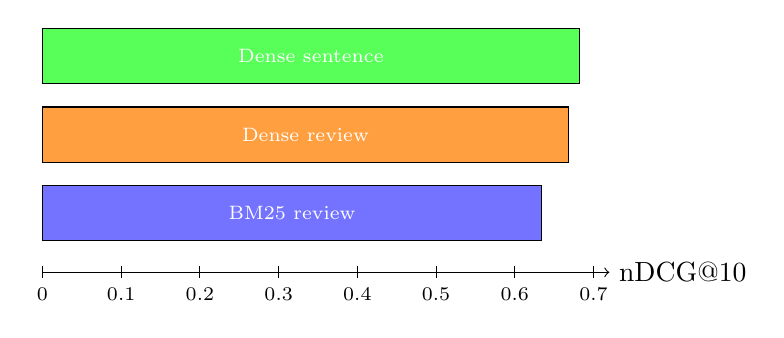
\begin{tikzpicture}[x=1cm,y=5cm]
\draw[->](0,0)--(7.2,0) node[right]{nDCG@10};
\foreach \x/\lab in {0/0,1/0.1,2/0.2,3/0.3,4/0.4,5/0.5,6/0.6,7/0.7}
  \draw(\x,0.015)--(\x,-0.015) node[below,font=\scriptsize]{\lab};
\draw[fill=blue!55](0,0.08) rectangle (6.34,0.22) node[midway,white,font=\scriptsize]{BM25 review};
\draw[fill=orange!75](0,0.28) rectangle (6.68,0.42) node[midway,white,font=\scriptsize]{Dense review};
\draw[fill=green!65](0,0.48) rectangle (6.82,0.62) node[midway,white,font=\scriptsize]{Dense sentence};
\end{tikzpicture}
\caption{Principal ranking configurations. Bars show the reported nDCG@10 means.}
\label{fig:principal-bars}
\end{figure}

\section{Aggregation and statistical comparison}
Dense retrieval beats BM25 under every review-level aggregation tested. The paired
dense-minus-BM25 nDCG@10 differences are:
\begin{table}[H]
\centering\small
\caption{Review-level dense versus BM25 comparison.}
\label{tab:significance}
\begin{tabular}{@{}lccc@{}}
\toprule
Aggregation & Difference & Holm-corrected $p$ & Significant\\
\midrule
Max & +0.050 & 0.009 & Yes\\
Mean & +0.094 & $<0.001$ & Yes\\
Top-3 mean & +0.053 & 0.003 & Yes\\
Top-5 mean & +0.047 & 0.009 & Yes\\
Top-10 mean & +0.035 & 0.020 & Yes\\
\bottomrule
\end{tabular}
\end{table}
The largest gap is for the plain mean because BM25 gives many nonmatching reviews a zero score.
Top-$k$ mean avoids dilution while using several pieces of evidence. Max is less stable because
one accidental match can determine the restaurant rank.

\section{Review-volume control}
Before control, top-10 score and review count correlate at approximately 0.30--0.36. After
capping every restaurant at 400 randomly sampled reviews, correlations are near zero and
nDCG changes by at most 0.011. The effect is visible in Figure~\ref{fig:volume}; it matters
for interpreting scores even when the final ranking changes modestly.
\begin{figure}[H]
\centering
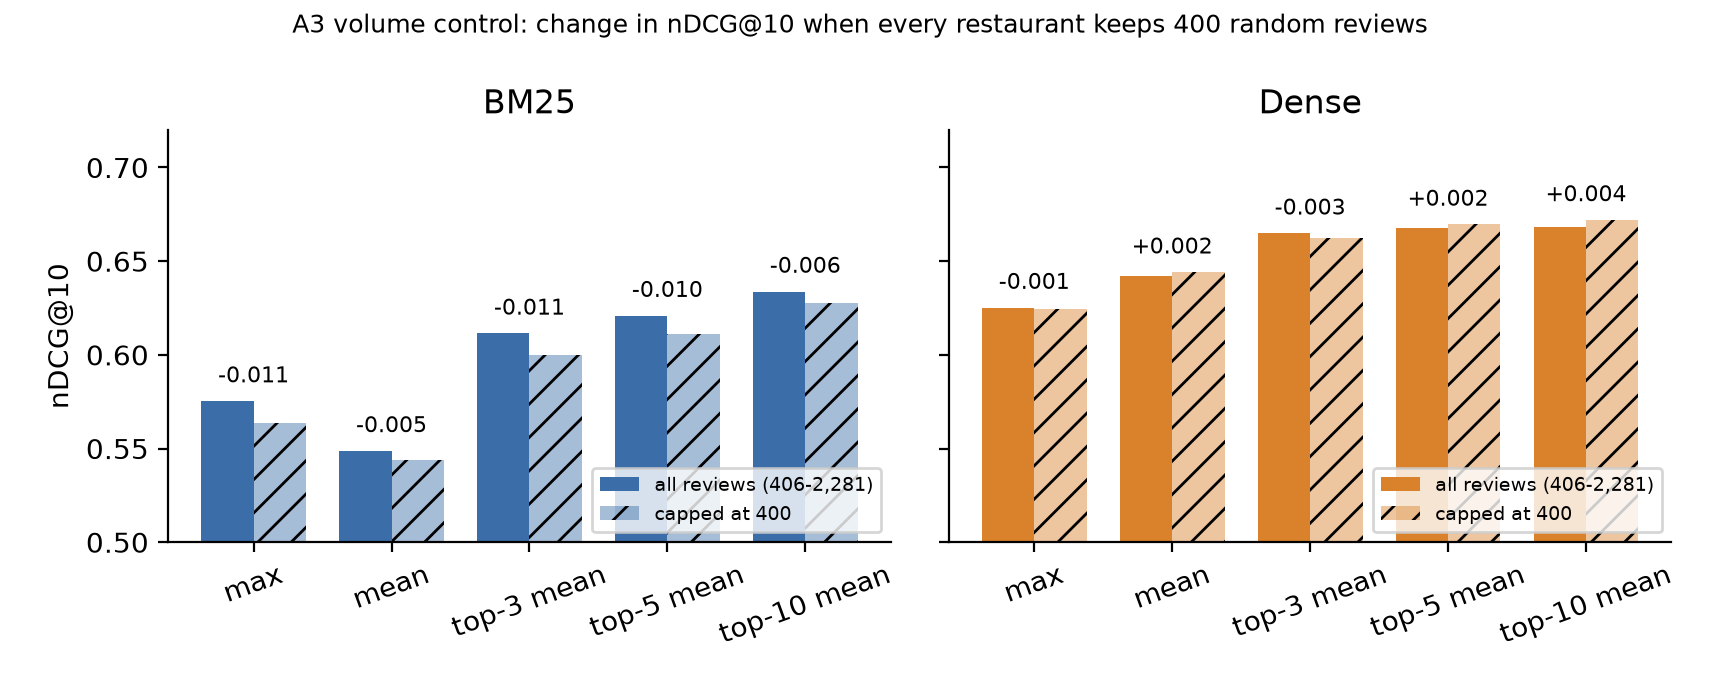
\includegraphics[width=\linewidth]{figures/a3_volume_control.png}
\caption{Effect of capping each restaurant at 400 reviews.}
\label{fig:volume}
\end{figure}

\section{B3 ablation and improvement results}
The experiments form a sequence of evidence-driven improvements:
\begin{enumerate}
\item sentence-level dense retrieval with top-10 mean increased nDCG@10 from 0.668 at review
level to 0.682;
\item volume control removed score/count correlations while changing nDCG by at most 0.011;
\item LLM rewriting and cross-encoder reranking were evaluated as an improved live pipeline.
\end{enumerate}
Applying rewriting and cross-encoder reranking to all 100 RIRD queries produced nDCG@10
0.658 and MAP 0.586, below the dense baseline. It improved 44 queries and degraded 53, with
mean nDCG change approximately $-0.024$. The largest gains were negation queries such as
``not Thai but Asian'' and ``not sushi but Asian'', while ordinary food and location queries
were often degraded. The likely cause is that the cross-encoder was trained for MS MARCO web
search rather than restaurant review relevance.

\begin{table}[H]
\centering\small
\caption{B3 ablation and deployment decision.}
\label{tab:b3}
\begin{tabular}{@{}lccp{5.0cm}@{}}
\toprule
Configuration & nDCG@10 & MAP & Decision\\
\midrule
Dense baseline & 0.682 & 0.618 & Keep for ordinary queries\\
Rewrite + CE for all queries & 0.658 & 0.586 & Do not use globally\\
Selective CE live rule & --- & --- & Use for explicit exclusions\\
\bottomrule
\end{tabular}
\end{table}

\section{Explanation and Thai evaluation}
The automatic deletion test found a mean faithfulness gap of 0.000 ($p=1.0$): shown and
random deletions were equally destructive because the evidence store was already pooled to the
top ten sentences per restaurant. This is a limitation of the test design, not evidence that
all explanations are good. The Thai pool contains 452 blind query--sentence pairs from 24
frozen taste queries. BM25 and dense top-ten pools overlap by only about 1.2 sentences on
average, providing complementary evidence for human assessment. Because restaurant IDs are
absent, Thai evaluation remains sentence-level and cannot be compared directly with RIRD
restaurant nDCG.
